\documentclass[tikz,border=6pt]{standalone}
\usepackage{tikz}
\usetikzlibrary{arrows.meta,calc}
\tikzset{
 planet/.style={draw,circle,minimum size=1.4cm,thick},
 force/.style={-Latex,very thick}
}
\begin{document}
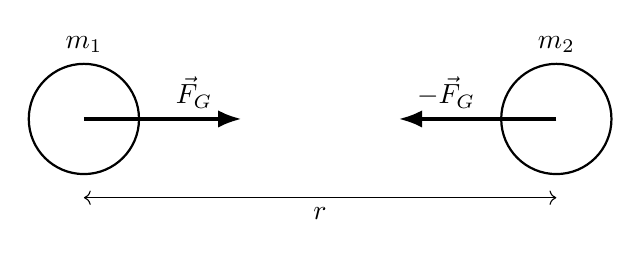
\begin{tikzpicture}
\node[planet,label=above:$m_1$] (m1) at (-3,0) {};
\node[planet,label=above:$m_2$] (m2) at (3,0) {};
\draw[force] (m1.center) -- ++(2,0) node[above,pos=.7] {$\vec{F}_{G}$};
\draw[force] (m2.center) -- ++(-2.0,0) node[above,pos=.7] {$-\vec{F}_{G}$};
\draw[<->] ($(m1.center)+(0,-1)$) -- node[midway,below] {$r$} ($(m2.center)+(0,-1)$);
\end{tikzpicture}
\end{document}
